\documentclass[12pt]{article}%
%Options -- Point size:  10pt (default), 11pt, 12pt
%        -- Paper size:  letterpaper (default), a4paper, a5paper, b5paper
%                        legalpaper, executivepaper
%        -- Orientation  (portrait is the default)
%                        landscape
%        -- Print size:  oneside (default), twoside
%        -- Quality      final(default), draft
%        -- Title page   notitlepage, titlepage(default)
%        -- Columns      onecolumn(default), twocolumn
%        -- Equation numbering (equation numbers on the right is the default)
%                        leqno
%        -- Displayed equations (centered is the default)
%                        fleqn (equations start at the same distance from the right side)
%        -- Open bibliography style (closed is the default)
%                        openbib

% general layout
\usepackage[dvips,letterpaper,margin=0.75in,bottom=0.75in]{geometry}
\usepackage{rotating}
%\usepackage{multicol}
\setlength{\parindent}{0pt}
\usepackage{setspace} % line spacing
\usepackage{changepage}

%\pagestyle{empty} % Removes page numbers
%\pagestyle{plain} 
\usepackage{fancyhdr}
\usepackage{lastpage}
\usepackage{extramarks}

% Setup the header and footer
\newcommand{\hmwkAuthorName}{Colin Leach}
\fancyhf{}
\pagestyle{fancy}                                                       %
\lhead{\hmwkAuthorName}                                                 %
\chead{\hmwkClass\ : \hmwkTitle}  %
\rhead{Page\ \thepage\ of\ \pageref{LastPage}}                          %
\renewcommand\headrulewidth{0.4pt}                                      %
\renewcommand\footrulewidth{0pt}                                      %

% Make title
\title{\vspace{-1cm}\textmd{\textbf{\hmwkClass:\ \hmwkTitle}}\\\normalsize\vspace{0.1in}\small{Due\ on\ \hmwkDueDate}\\\vspace{0.1in}}
\date{}
\author{\textbf{\hmwkAuthorName}}\vspace{-0.2in}

% base encodings
\usepackage[utf8]{inputenc}
\usepackage[T1]{fontenc}

% math support packages
\usepackage{amsmath}
\usepackage{amsfonts}
\usepackage{amssymb}
\usepackage{mathabx}
%\usepackage[retainorgcmds]{IEEEtran} % problems installing with MikTeX
\DeclareMathOperator{\tr}{tr} % trace of a matrix
\usepackage{mathptmx}
%\usepackage{newtxmath}
\usepackage{bm} % bold math
%\usepackage{commath}
\usepackage{mathtools}
\usepackage{upgreek}
\DeclareMathAlphabet{\mathcal}{OMS}{cmsy}{m}{n}


% graphics-related packages and settings
\usepackage{graphicx}
\graphicspath{ {images/} }
\usepackage{wrapfig} % allow text to wrap around (narrow) figures
%\usepackage{float} % do not use with floatrow
\usepackage{floatrow} % allow floats and captions side by side
\usepackage[font=small,labelfont=bf,labelsep=space,justification=raggedright]{caption}
\usepackage{chngcntr} % defines \counterwithin and \counterwithout
\counterwithin{figure}{section}

% table formatting
\usepackage{makecell}
\usepackage[table]{xcolor}
\usepackage{array} % wrap within tables
\newcolumntype{L}{>{\centering\arraybackslash}m{12cm}}

% miscellaneous
\usepackage{subfiles} % include source from separate files
\usepackage{hyperref} % hypertext support
\usepackage{color}
\usepackage[bottom]{footmisc}
\newcommand{\tsub}[1]{\textsubscript{#1}}
\newcommand{\tsup}[1]{\textsuperscript{#1}}
\newcommand{\so}{\qquad \implies \qquad}
\newcommand{\todo}{\color{red}{TODO}\color{black}\hspace{2mm}}

% for software source code
% Python, Matlab, etc are built in as atandard but Julia needs to be added here
\usepackage{listings}
%%
%% Julia definition (c) 2014 Jubobs
%%
\lstdefinelanguage{Julia} 
{morekeywords={abstract,break,case,catch,const,continue,do,else,elseif,%
		end,export,false,for,function,immutable,import,importall,if,in,%
		macro,module,otherwise,quote,return,switch,true,try,type,typealias,%
		using,while},%
	sensitive=true,%
	alsoother={$},%
	morecomment=[l]\#,%
	morecomment=[n]{\#=}{=\#},%
	morestring=[s]{"}{"},%
	morestring=[m]{'}{'},%
}[keywords,comments,strings]%






%\setlength{\headsep}{-10pt}
\setlength{\parskip}{0.2em}
%\setlength{\textheight}{11 in}
\setlength{\skip\footins}{20pt}

% Homework Specific Information
\newcommand{\hmwkClass}{ASTR 400B}
\newcommand{\hmwkTitle}{Homework 3}
\newcommand{\hmwkDueDate}{Feb 6, 2020}

\hyphenpenalty=1000

\begin{document}
	
\maketitle

\section*{2. Mass Breakdown}

This is raw output from pandas.DataFrame.to\_latex(), with rows sorted alphabetically:\\

\begin{tabular}{lccccc}
	\toprule
	Galaxy Name &  Halo Mass &  Disk Mass &  Bulge Mass &  Total &  f\_bar \\
	\midrule
	M31 &      1.921 &      0.120 &       0.019 &  2.060 &  0.068 \\
	M33 &      0.187 &      0.009 &       0.000 &  0.196 &  0.047 \\
	MW &      1.975 &      0.075 &       0.010 &  2.060 &  0.041 \\
	All &      4.082 &      0.204 &       0.029 &  4.316 &  0.054 \\
	\bottomrule
\end{tabular}\vspace{5mm}

With a bit of manual formatting:\\

\begin{tabular}{lccccc}
	\toprule
	\textbf{Galaxy Name} &  \textbf{Halo Mass}  &  \textbf{Disk Mass} &  \textbf{Bulge Mass} &  \textbf{Total} &  $\mathbf{f_{bar}}$ \\
	 & ($M_\Sun \times 10^{12}$) & ($M_\Sun \times 10^{12}$) & ($M_\Sun \times 10^{12}$) & ($M_\Sun \times 10^{12}$) & \\
	\midrule
	MW &  1.975 &  0.075 &   0.010 &  2.060 &  0.041 \\
	M31 &  1.921 &  0.120 &   0.019 &  2.060 &  0.068 \\
	M33 &  0.187 &  0.009 &   0.000 &  0.196 &  0.047 \\
	\midrule
	Local Group &  4.082 &  0.204 &   0.029 &  4.316 &  0.054 \\
	\bottomrule
\end{tabular}\vspace{5mm}

Compare that with particle counts:\\

\begin{tabular}{lrrrrr}
	\toprule
	\textbf{Galaxy Name} &  \textbf{Halo Count}  &  \textbf{Disk Count} &  \textbf{Bulge Count} &  \textbf{Total} \\
	\midrule
	MW   &   50000 &   75000 &    10000 &  135000 \\
	M31  &   50000 &  120000 &    19000 &  189000 \\
	M33  &    5000 &    9300 &        0 &   14300 \\
	\midrule
	All  &  105000 &  204300 &    29000 &  338300 \\
	\bottomrule
\end{tabular}\vspace{5mm}

The DM halo contains fewer but more massive particles. This may be easier to see on stacked bar charts showing the distribution:

{\centering 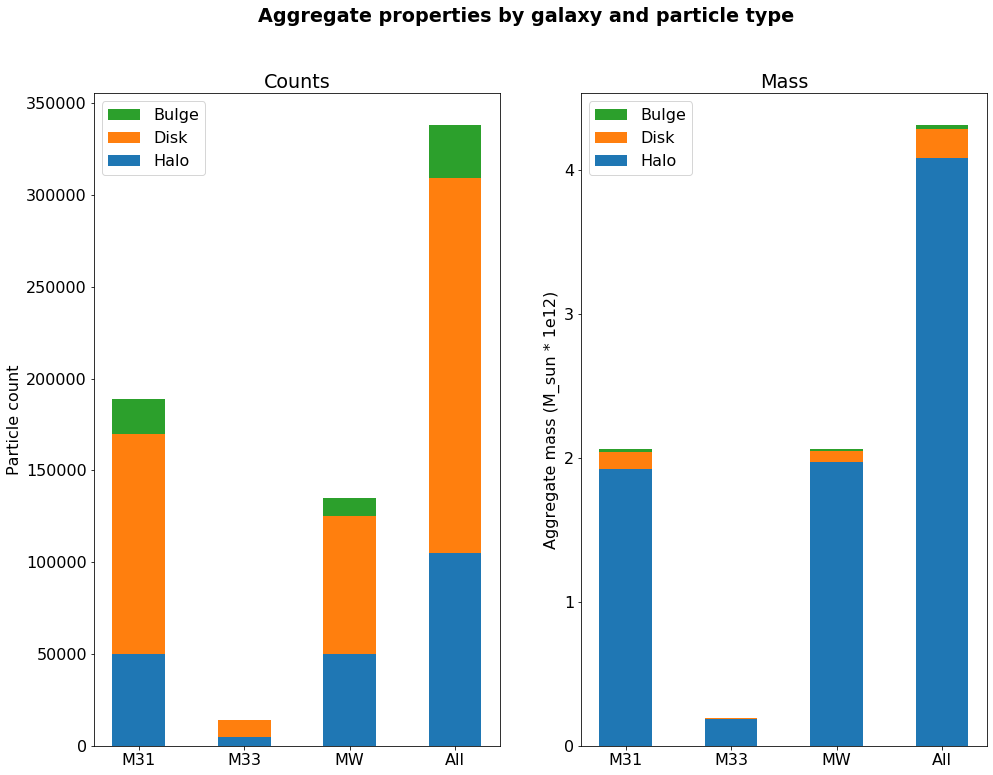
\includegraphics[scale=0.5]{stackedbar} \par}

\section*{3. Questions}

\paragraph{1. Total mass:} M31 and the MW have the same total mass in this simulation. Dark matter in the halo dominates in most cases, but especially for the MW.

\paragraph{2. Stellar mass:} Disk + bulge mass is about 60\% higher for M31 than the MW. Assuming a roughly similar distribution of star types and ages, M31 is likely to be more luminous.

\paragraph{3. Dark matter mass:} 

\paragraph{4. Baryon fraction:} 

\end{document}
